\section{Evaluation} \label{sec-evaluation} 
In this section, we evaluate the performance of our proposed optimizations.
\subsection{Setup}
To evaluate our proposed optimizations, we provide two different set of workloads, namely, OpenML workload and Kaggle workload.

\textbf{OpenML workloads.} In the OpenML workloads, we utilize some of the popular machine learning pipelines from the OpenML repository for solving task 31, i.e., classifying customers as good or bad credit risks using the German Credit data from the UCI repository \cite{Dua:2017}\footnote{https://www.openml.org/t/31}.
Table \ref{tab-openml-pipelines} shows the id, components, and number of executions of the OpenML pipelines.\footnote{information about each pipeline is available at https://www.openml.org/f/id}
\begin{table}
\begin{tabular}{llr}
\hline
\textbf{id} & \textbf{operations} & \textbf{\#exec}   \\
\hline
 5981&  \makecell[l]{Imputer\rightarrow Standard scaler\rightarrow Logistic regression} &11        \\
 7707&  \makecell[l]{Imputer\rightarrow Onehot encoder \rightarrow Standard scaler\\ \rightarrow Variance thresholder \rightarrow SVM }&594 \\
 8315&  \makecell[l]{Imputer\rightarrow Onehot encoder\rightarrow Variance thresholder\\ \rightarrow Random Forest} &1084  \\
8353 & \makecell[l]{Imputer\rightarrow Onehot encoder\rightarrow Variance thresholder \\ \rightarrow Svm}  & 1000\\
8568 &  \makecell[l]{Imputer\rightarrow Onehot encoder\rightarrow Variance thresholder \\ \rightarrow Random Forest} &555 \\
\hline
\end{tabular}
\caption{OpenML pipeline descriptions.}
\vspace{-25pt}
\label{tab-openml-pipelines}
\end{table}

\textbf{Kaggle workloads.} In the second set of workloads, we target interactive machine learning loads where a large portion of the analysis is spent on data and feature preprocessing.
We design the workload by studying several Kaggle scripts and populating the database based on those.
Here's the description of the Kaggle challenges that we use.
\todo[inline]{This is my next immediate ToDo.}

\subsection{Reuse and Warmstarting for the OpenML Workload}
\subsubsection{Feature Processing Reuse}  
In Figure \ref{evaluation-reuse-open-figure}, we show the effect of the reuse optimization on the OpenML workflow.
The number of executed steps drastically decreases as the majority of the pipelines have the exact same data transformation steps and they only differ in the hyperparameters of the model (Figure \ref{evaluation-reuse-open-figure}a).
However, Figure \ref{evaluation-reuse-open-figure}b shows that the reuse optimization does not impact the total execution time.
This is specific to the OpenML use case, as the model training time dominates the data transformation time.
\todo[inline]{The figure only shows estimates}

\begin{figure}
\centering
\begin{subfigure}{.5\linewidth}
  \includegraphics[width=\linewidth]{../images/experiment-results/reuse-openml-steps.eps}
  \caption{Executed Steps}
  \label{fig:sub1}
\end{subfigure}%
\begin{subfigure}{.5\linewidth}
  \includegraphics[width=\linewidth]{../images/experiment-results/reuse-openml-time.eps}
  \caption{Execution Time}
  \label{fig:sub1}
\end{subfigure}
\caption{Effect of the reuse optimization on the total number of executed transformations and the total execution time for every OpenML pipeline}
\label{evaluation-reuse-open-figure}
\end{figure}

\subsubsection{Model Warmstarting}
In this experiment, we study the effect of the model warmstarting optimization on two pipelines (pipelines 5891 and 8568) from the openml database.
Pipeline 5891 has a logistic regression model.
There a total of 11 configurations in the database.
The stopping condition for the logistic regression model is the convergence tolerance.
Pipelines 8568 has random forest model.
There are a total 555 configurations for pipelines 8568.
The training of the random forest stops when the number of samples in any leaf node is below a user-defined threshold.

Figure \ref{evaluation-warmstarting-figure} shows the result of the model warmstarting optimization on two types of models in the experiment database.
Figures \ref{evaluation-warmstarting-figure}a and \ref{evaluation-warmstarting-figure}b shows the effect of warmstarting on the logistic regression model.
Since the data size is small, the training time is fast and the total time is mostly dominated by the data processing and start-up time.
To better show the effect of the warmstarting on the model training, we also include the total number of iterations for training the model on all 11 configurations.
The warmstarting optimization reduces the number of iterations by a factor of three.
Figure \ref{evaluation-warmstarting-figure}c shows the total training time for all the 555 random forest models.
The warmstarting optimization reduces the total training time by one order of magnitude (from 300 seconds to 30 seconds).

\begin{figure}
\centering
\begin{subfigure}{.5\linewidth}
  \includegraphics[width=\linewidth]{../images/experiment-results/warmstarting-lr-5981-runtime.eps}
  \caption{total training time (lr)}
  \label{fig:sub1}
\end{subfigure}%
\begin{subfigure}{.5\linewidth}
  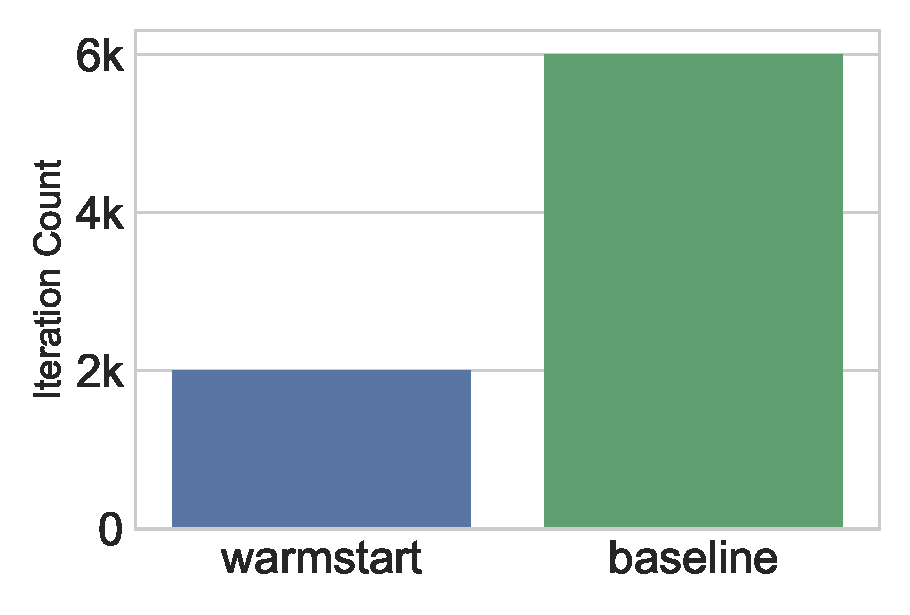
\includegraphics[width=\linewidth]{../images/experiment-results/warmstarting-lr-5981-iterations.eps}
  \caption{total iteration count (lr)}
  \label{fig:sub1}
\end{subfigure}
\begin{subfigure}{.5\linewidth}
  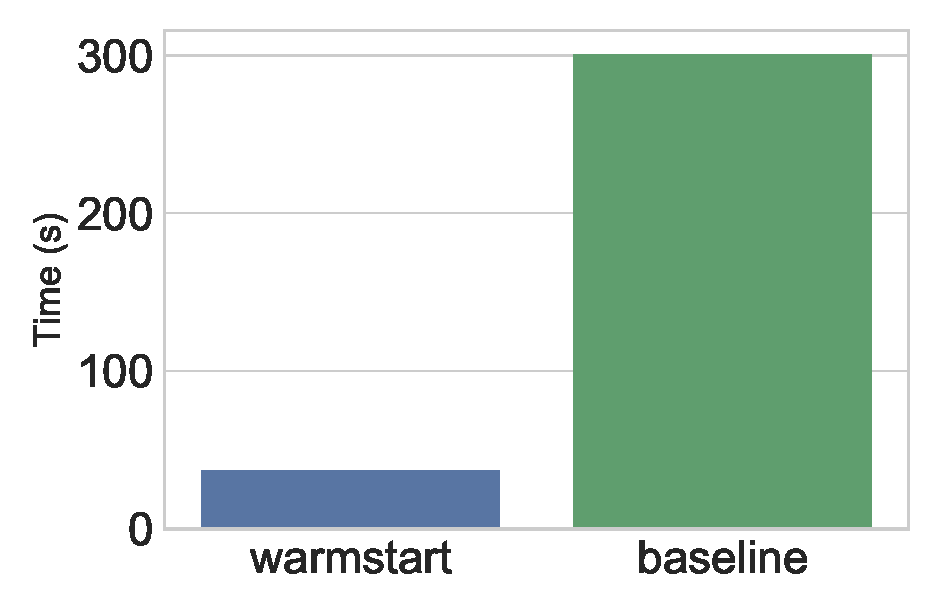
\includegraphics[width=\linewidth]{../images/experiment-results/warmstarting-rf-8568-time.eps}
  \caption{total training time (rf)}
  \label{fig:sub1}
\end{subfigure}
\caption{Effect of the warmstarting optimization on the total training time and iteration count. In (a) and (b) we train 11 logistic regression models and in (c) we train 555 random forest model from the configurations that exist in the experiment data.}
\label{evaluation-warmstarting-figure}
\end{figure}

\subsubsection{Partial Warmstarting}

\subsubsection{Combined Optimization}
In this section we study the effect of combining all three optimizations (feature processing reuse, warmstarting, and partial warmstarting).

\subsection{Reuse and Warmstarting for the Interactive Workload}

\subsection{Evaluation of Optimizing the Hyperparameter Search}
\todo[inline]{These results are still without the 'Avoiding Local Optima' solution, so ideally, once we find a good solution to avoid local optimas we should get even better results.}

In this experiment, we focus on several of the popular machine learning pipelines (flow 7707, 8353, 8315) designed for solving task 31\footnote{https://www.openml.org/t/31}, classifying customers as good or bad credit risks using the German Credit data from the UCI repository \cite{Dua:2017}.
We extracted the meta-data from the OpenML database which includes all the executions of the pipeline, the value of the hyperparameters, and the evaluation metrics.
Using the meta-data, we initialize the hyperparameter optimization process with the values of the hyperparameters for each execution and the loss ($1- accuracy$) for the specific execution.
We then execute the search with a budget of 100 trials, trying to minimize the loss of the OpenML pipelines.
We repeat this experiment 10 times, for every pipeline.
Figure \ref{fig-avg-warm-vs-cold-task-31} shows the average of losses of the 100 trials for the 10 experiments.
Warm starting the search decreases the overall loss of the trials.

\begin{figure}
\centering
\includegraphics[width=\columnwidth]{../images/experiment-results/task31-cold-warm-trials.eps}
\caption{Loss value of 100 Trials with and without warmstarting}
\label{fig-avg-warm-vs-cold-task-31}
\end{figure}

\subsection{Avoiding Local Optima}

\subsubsection{Adaptive Selection}
In this experiment, we show the result of our adaptive selection methods on the hyperparameter search process.
Figure \ref{fig-avg-adaptive-selection-task-31} shows the result of the histogram and random selection method on the hyperparameter search process.
When compared to the vanilla approach (where full history is used in warmstarting), we see that random selection decrease the error rate of the trials where histogram increases them.
To make the difference more visible we limit the scope of the loss (y axis) from 0.20 to 0.25.
\begin{figure}
\centering
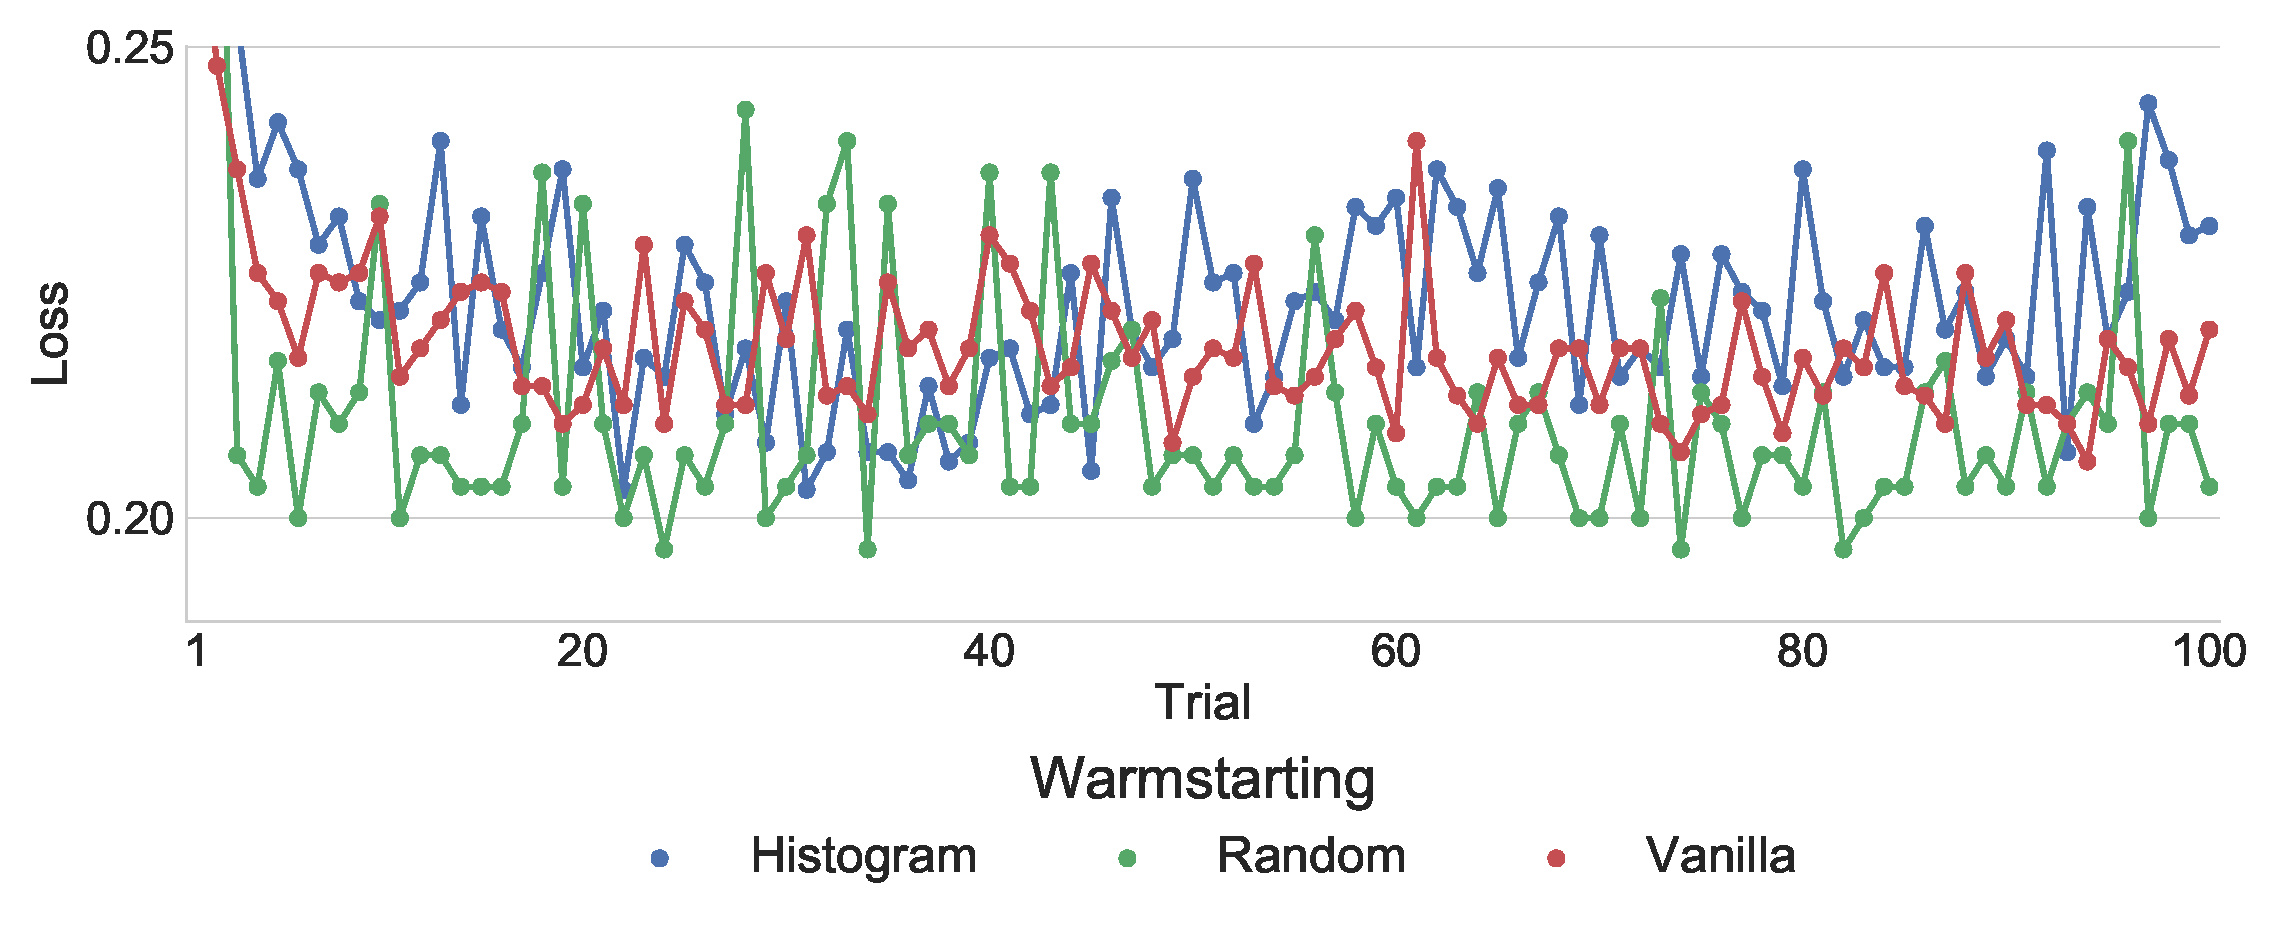
\includegraphics[width=\columnwidth]{../images/experiment-results/t31-f7707-adaptive-method-random.eps}
\caption{Effect of adaptive warmstarting on hyperparameter search process}
\label{fig-avg-adaptive-selection-task-31}
\end{figure}

\begin{table}
\centering
\begin{tabular}{crrr}
\hline
	   Pipeline & Best Loss & Warm & Cold \\ \hline
        7707 & 0.16 & 1 & 0 \\
        8315 & 0.18 & 173 & 14\\
        8353 & 0.18 &0& 1\\ 
        8568 & 0.15 &0&2\\
        \hline
\end{tabular}
\caption{Best loss and their occurrences for different pipelines using warm starting}
\end{table}

%Table \ref{table-best-hyperparameters} shows the best loss achieved from the search process for every pipeline on the Task 31.
%Figure \ref{figure-best-hyperparameters} shows the number of time that the search process (with budget of 100) manages to find the best set of hyperparameters that results in the lowest loss value.
%While both with and without warm starting does find the best set of hyperparameters, using warmstarting outperforms the search without wamrstarting and has a higher probability of finding the best hyperparameters.
%
%\begin{minipage}{\columnwidth}
%  \begin{minipage}[m]{0.49\columnwidth}
%   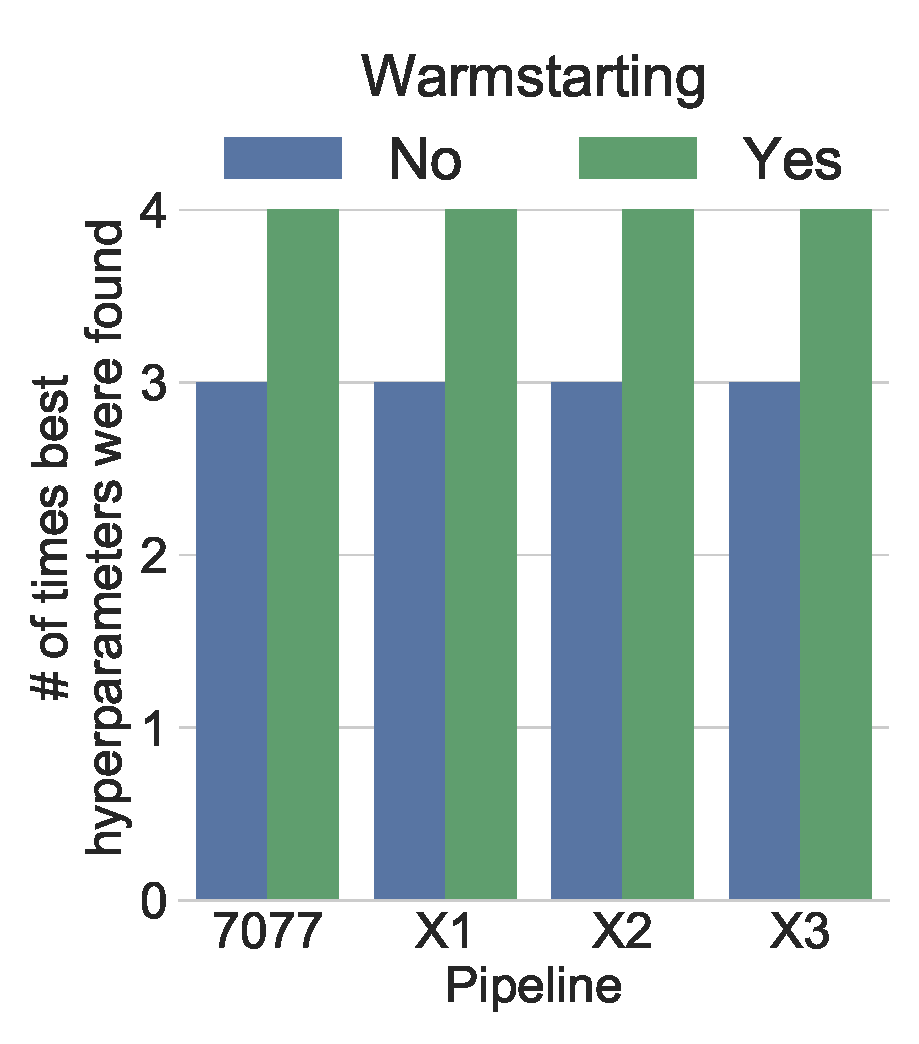
\includegraphics[width=\columnwidth]{../images/experiment-results/task31-cold-starting-warm-besthyperparametersfound.eps}
%    \captionof{figure}{Occurrences of best hyperparameters}
%     \label{figure-best-hyperparameters}
%  \end{minipage}
%  \hspace{0.5cm}
%  \begin{minipage}[m]{0.49\columnwidth}
%    \begin{tabular}{cc}\hline
%      Pipeline & Best Loss \\ \hline
%        7077 & 0.189 \\
%        X1 & XXX \\
%        X2 & XXX \\ \hline
%      \end{tabular}
%      \captionof{table}{Best hyperparameters}
%      \label{table-best-hyperparameters}
%    \end{minipage}
%  \end{minipage}
%\subsection{Data Materialization}